\documentclass{standalone}
\usepackage{tikz}
\usepackage{ctex,siunitx}
\setCJKmainfont{Noto Serif CJK SC}
\usepackage{tkz-euclide}
\usepackage{amsmath,mhchem}
\usetikzlibrary{patterns, calc}
\usetikzlibrary {decorations.pathmorphing, decorations.pathreplacing, decorations.shapes,}
\begin{document}
\small
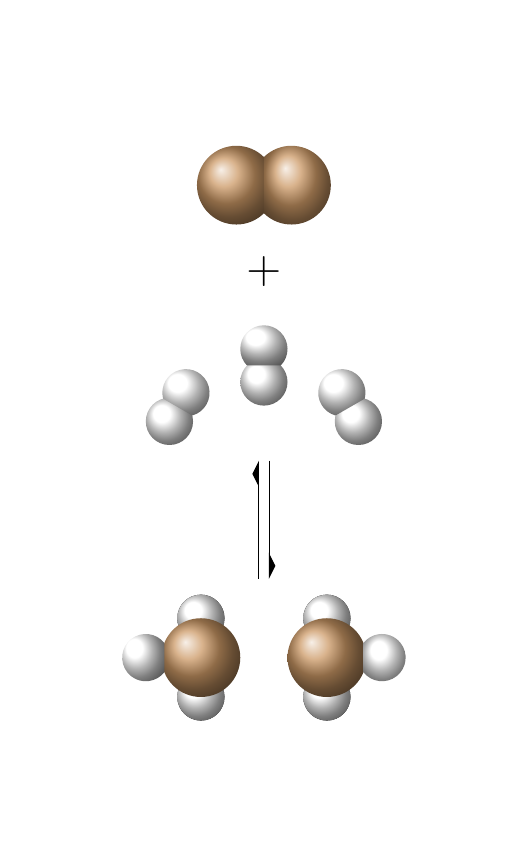
\begin{tikzpicture}[>={Diamond[left,scale=1.5]},scale=1.0]
  \useasboundingbox(-3,2)rectangle(3,-8);
  \begin{scope}[xshift=-3.5mm]
    \tkzDefPoints{0/0/O,0/0.5/R,0.7/0/H1,1.2/0/r1}
    \tkzInterCC(O,R)(H1,r1)\tkzGetPoints{A}{B}
    \tkzDrawCircle[draw=none,ball color=brown!80](O,R)
    \tkzDrawArc[draw=none,ball color=brown!80](H1,B)(A)
  \end{scope}
  \begin{scope}[yshift=-2.5cm,rotate=90,scale=0.6]
    \tkzDefPoints{0/0/O,0/0.5/R,0.7/0/H1,1.2/0/r1}
    \tkzInterCC(O,R)(H1,r1)\tkzGetPoints{A}{B}
    \tkzDrawCircle[draw=none,ball color=white](O,R)
    \tkzDrawArc[draw=none,ball color=white](H1,B)(A)
  \end{scope}
  \begin{scope}[xshift=12mm,yshift=-3cm,rotate=120,scale=0.6]
    \tkzDefPoints{0/0/O,0/0.5/R,0.7/0/H1,1.2/0/r1}
    \tkzInterCC(O,R)(H1,r1)\tkzGetPoints{A}{B}
    \tkzDrawCircle[draw=none,ball color=white](O,R)
    \tkzDrawArc[draw=none,ball color=white](H1,B)(A)
  \end{scope}
  \begin{scope}[xshift=-12mm,yshift=-3cm,rotate=60,scale=0.6]
    \tkzDefPoints{0/0/O,0/0.5/R,0.7/0/H1,1.2/0/r1}
    \tkzInterCC(O,R)(H1,r1)\tkzGetPoints{A}{B}
    \tkzDrawCircle[draw=none,ball color=white](O,R)
    \tkzDrawArc[draw=none,ball color=white](H1,B)(A)
  \end{scope}
  \node at (0,-1.1){\LARGE $+$};
  \draw[->](0.07,-3.5)--++(0,-1.5);
  \draw[<-](-0.07,-3.5)--++(0,-1.5);
  \begin{scope}[xshift=-8mm,yshift=-6.0cm]
    \tkzDefPoints{0/0/O,0/0.5/R,-0.7/0/H1,-1/0/r1}
    \tkzInterCC(O,R)(H1,r1)\tkzGetPoints{A}{B}
    \fill[ball color=white](0,0.5)circle(0.3);
    \fill[ball color=white](0,-0.5)circle(0.3);
    \tkzDrawCircle[draw=none,ball color=brown!80](O,R)
    \tkzDrawArc[draw=none,ball color=white](H1,B)(A)
  \end{scope}
  \begin{scope}[xshift=8mm,yshift=-6.0cm,rotate=180]
    \tkzDefPoints{0/0/O,0/0.5/R,-0.7/0/H1,-1/0/r1}
    \tkzInterCC(O,R)(H1,r1)\tkzGetPoints{A}{B}
    \fill[ball color=white](0,0.5)circle(0.3);
    \fill[ball color=white](0,-0.5)circle(0.3);
    \tkzDrawCircle[draw=none,ball color=brown!80](O,R)
    \tkzDrawArc[draw=none,ball color=white](H1,B)(A)
  \end{scope}
  
\end{tikzpicture}
\end{document}